

\renewcommand{\familydefault}{cmss}

\definecolor{fgcgray}{rgb}{0.4, 0.4, 0.4}
\definecolor{darkblue}{rgb}{0,0, 0.4}
\newcommand{\titlefont}[1]{\textcolor{black}{\fontseries{bx}\fontshape{n}\fontsize{30}{0pt} \selectfont #1}}
\newcommand{\titlepagef}[1]{\textcolor{black}{\fontseries{bx}\fontshape{n}\fontsize{14}{0pt} \selectfont #1}}

\newcommand{\gloss}[1]{\textcolor{glossb}{\fontsize{11}{0pt}\selectfont #1}}



\addtolength{\oddsidemargin}{-1.0cm}
\addtolength{\evensidemargin}{-1.0cm}
\addtolength{\headwidth}{2.0cm}
\addtolength{\textwidth}{2.0cm}

\setlength{\parindent}{0cm}

\renewcommand{\labelitemi}{$\circ$}
\renewcommand{\labelitemii}{$\diamond$}

\newcommand{\spaceline}[1][8pt]{\vskip #1}
\newcommand{\attrname}[1]{\textcolor{fgcgray}{\scriptsize #1}}

\newcommand{\comment}[1]{\spaceline[5pt] \textcolor{fgcgray}{\scriptsize #1} \spaceline[15pt]}

\makeatletter

\newcommand*{\project}[1]{\gdef\@project{#1}}


\def\@maketitle{
  %\begin{titlepage}
   
  \begin{center}
      \titlepagef{Softwareprojekt 2017}
      \spaceline
  \end{center}
  
  \begin{center}
      \parbox{\textwidth}{
        \spaceline
        \centering{\titlefont{Grobentwurf:\\ Realtime Mesh Utilities}}
        \par
        \spaceline
      }
  \end{center}
  
  \begin{center}
  \begin{tabbing}
  Petros Simiday \qquad \=
  Blerta Hamzallari \qquad \=
  Felix Griesau \qquad \=
  Marco Klamke \\
  Julius Lerm
  \>Lars Debor
  \>Sugandha Sachdeva  
  \>Simon Heinke
  \end{tabbing}
  \end{center}
 
  
  \spaceline[3em] {
    \begin{flushright}
    \begin{tabular}[t]{rl}
      \attrname{letzte Änderung:} & \@date
    \end{tabular}
    \end{flushright}
    \par
  }
  \spaceline[5.5em]
  %\end{titlepage}
}

\begin{document}
	
\lhead{\sc{Preliminary Design: RTMU}}	
\title{Preliminary Design: RTMU}
\vspace{3 in}
\maketitle
\clearpage

\tableofcontents

\clearpage
\section{The MNE-CPP Framework}

\subsection{Basic Structure of MNE-CPP}

MNE-CPP is a framework of tools and programs to analyze and work with MEG/EEG data.
It provides a cross-platform library which allows the processing of the in neuroscience well established Elekta Neuromag® FIFF file format and therefore integrates with existing toolboxes. \\
Besides the library, the MNE-CPP framework so far includes three main applications: MNE-Analyze, which centers around visualization of preprocessed data; MNE-Browse, which allows browsing raw data, e.g. FIFF files in a convenient way and MNE-Scan, which deals with acquiring and processing data. \\
The library itself consists of a collection of packages that provide interfaces for file handling, device connectivity, 2D- and 3D-visualization and mathematics.

\subsection{Integration of the Product into MNE-CPP}

The real-time mesh utilities are to be integrated into the structure of the MNE-CPP framework. To provide a versatile interface, the utilities are organized inside a package within the library layer (see figure 1). Later on, the features are to be ported to MNE-Scan, so they can be used within the application.
\begin{figure}[h]
	\begin{center}
		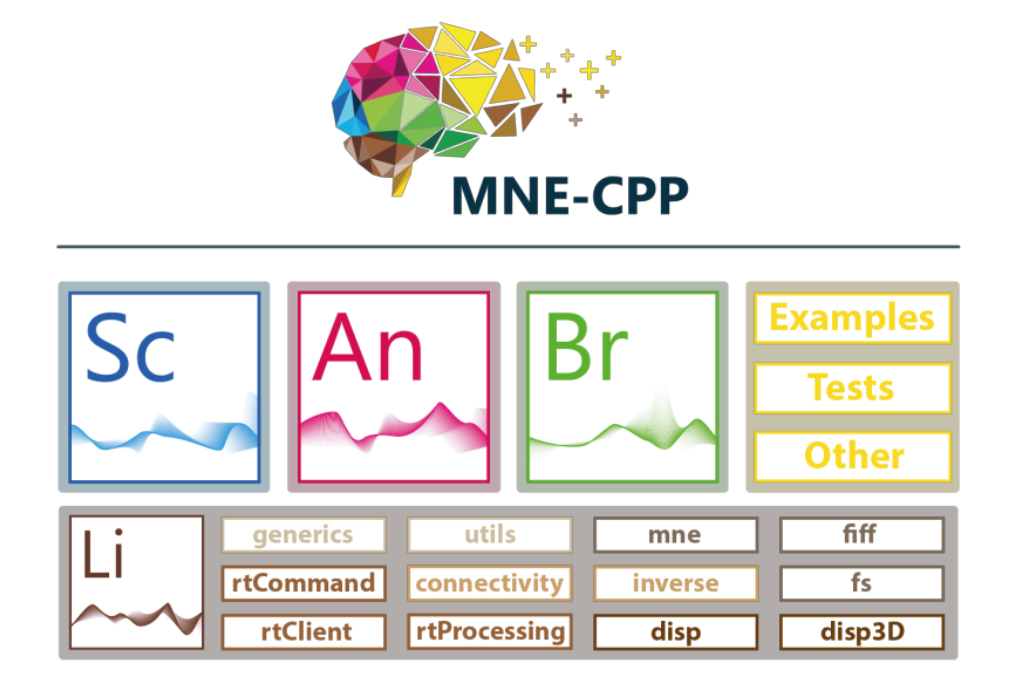
\includegraphics[width=10cm]{figures/mne_architecture.png}
		\caption{Overview of the MNE-CPP basic architectural layout, including application and library layer.}
	\end{center}
\end{figure}

\clearpage

\section{Subdivision of Program Features}

\begin{aims}
	
	\item[SCDC] 
	The surface constrained distance calculation algorithm receives a mesh data set as its input, which is stored inside a file. It then calculates approximate distances between vertices. When no further input arguments are provided, the SCDC algorithm calculates a full distance table, i.e. the distance between any vertex to any other vertex.
	When it receives a subset of the vertices as an additional argument, it only calculates the distances from said subset to every other vertex of the mesh. The SCDC algorithm stores its results inside a two-dimensional matrix.
	
	\item[Projecting]
	The projecting algorithm maps MEG/EEG-sensors to vertices of the mesh. In case of MEG-sensors, the orientation is known and thus a radial projection is applied in order to assign each sensor to a vertex. In case of EEG-sensors, the orientation is not known and a nearest-neighbor algorithm is used.
	The projecting algorithm then outputs the results of the calculation as an array of indices, which point to the respective vertices of the mesh.
	
	\item[Interpolation]
	The interpolation algorithm uses the results of both the projecting algorithm and the SCDC algorithm.
	Based on the distance table, it calculates a weight matrix for the later live interpolation. 
	Thus the interpolation algorithm receives three different inputs: the distance table created by SCDC, the sensors mapping and the actual sensor input, i.e. brain activity recorded by sensors over a period of time.
	The recorded brain activity gets passed to the interpolation algorithm either from an ongoing MEG/EEG-Scan or a prerecorded data set, i.e. a file. 
	
	\item[Disp3D]
	In order to provide control over aspects of the interpolation within the MNE-CPP framework, a new function is added to the Disp3D tree model.
		
\end{aims}

By dividing the real-time mesh utilities into the mentioned components, internal changes and extensions are easy to implement. Added to that, the single components can be reused elsewhere within the MNE-CPP framework.

\clearpage

\section{Basic Structure and Interface}

\begin{aims}
	\item[GeometryInfo] To provide the highest possible level of usability and versatility, a function to calculate surface constrained distances as well as the sensor-to-mesh mapping can be found inside the class \textit{GeometryInfo}. The mentioned option to provide a subset of vertices for the SCDC can be omitted by passing an empty vector as the second argument. 

\begin{figure}[h]
	\begin{center}
		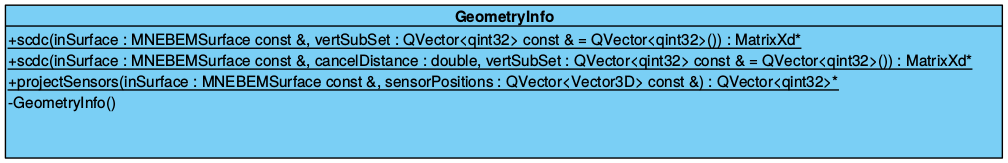
\includegraphics[width=16cm]{figures/geometryinfoclassdiagram.png}
		\caption{Interface of GeometryInfo}
	\end{center}
\end{figure}

\item[Interpolation] In order to keep the interpolation of neurophysiological activity efficient, the mentioned weight matrix (see section 2) is stored as a member of type MatrixXd inside the class \textit{Interpolation}, or rather as a pointer to such.
To use the precalculated weight matrix, one has to pass the current set of sensor data to the function \textit{interpolateSignals} and receives the results as a vector.

\begin{figure}[h]
	\begin{center}
		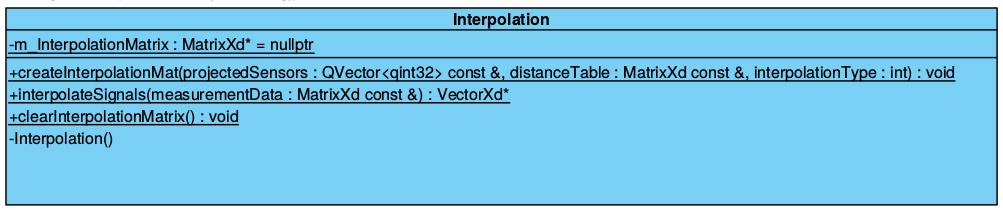
\includegraphics[width=16cm]{figures/interpolationclassdiagram.png}
		\caption{Interface of Interpolation}
	\end{center}
\end{figure}

\clearpage

\item[SensorDataTreeItem] To achieve the mentioned integration into the GUI framework, the program must integrate the SensorDataTreeItem.

\begin{figure}[h]
	\begin{center}
		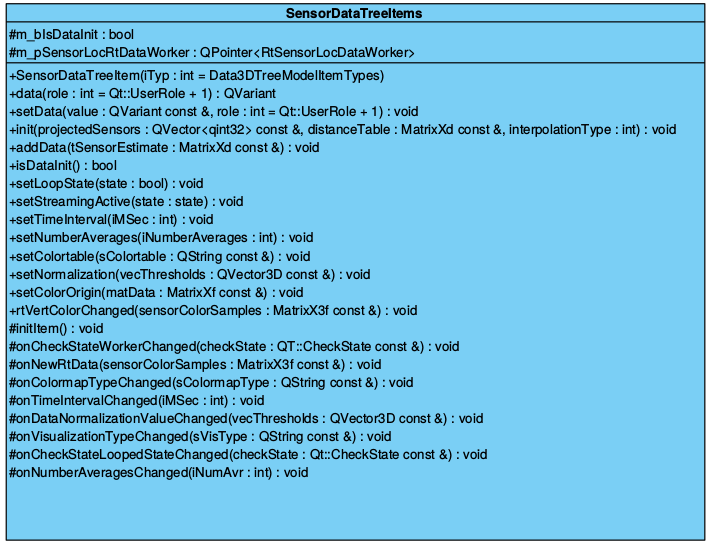
\includegraphics[width=16cm]{figures/sensordatatreeitemclassdiagram.png}
		\caption{SensorDataTreeItem}
	\end{center}
\end{figure}

\end{aims}

\begin{figure}[h]
	\begin{center}
		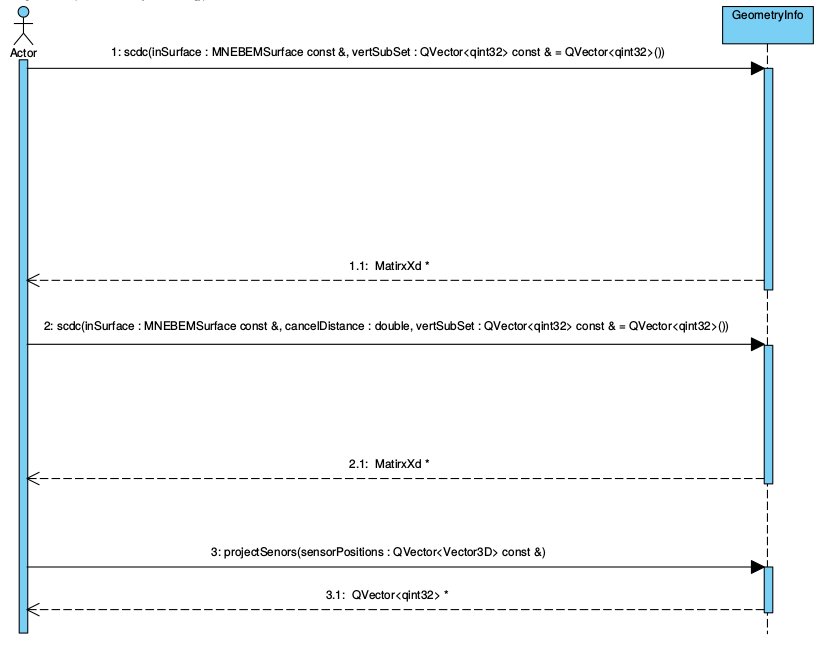
\includegraphics[width=16cm]{figures/geometryinfo_calling_sequence.png}
		\caption{Geometry calling sequence}
	\end{center}
\end{figure}

\begin{figure}[h]
	\begin{center}
		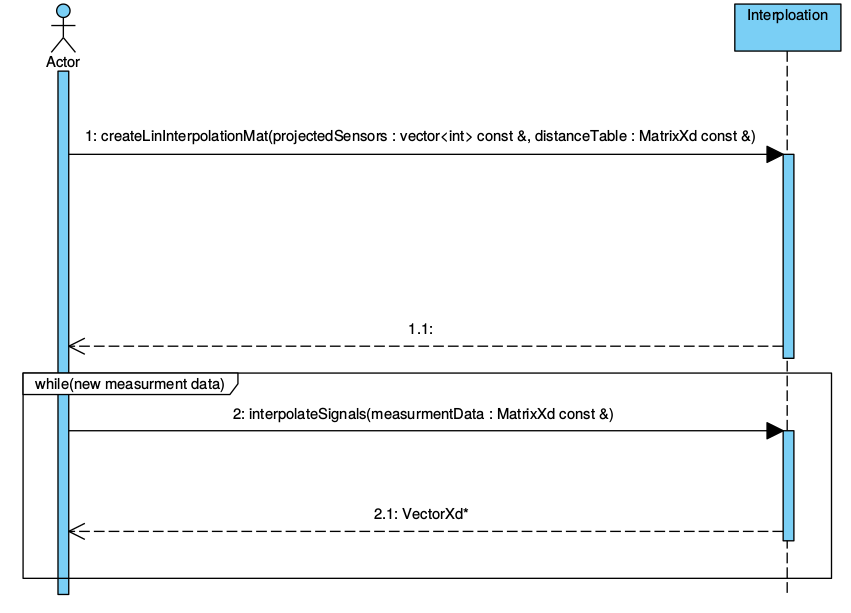
\includegraphics[width=16cm]{figures/interpolation_calling_sequence.png}
		\caption{Interpolation calling sequence}
	\end{center}
\end{figure}

\clearpage
  
\end{document}
